%!TEX root = ../Thesis.tex

\chapter{Selección de modelo}

\epigraphhead[70]{
\epigraph{Choose well. Your choice is brief, and yet endless.}
{Johann Wolfgang von Goethe}}

Puesto que el problema abarca también el detectar cuántos personas están involucrados en la grabación, y hasta ahora se ha considerado que se dispone de esta información, es necesario inferir de alguna manera cuántos interlocutores participan.

La contribución principal de este trabajo de tesis está en la selección de modelo propuesta, utilizando varias técnicas tanto bayesianas como frecuentistas para respaldar la elección realizada.

Como mencionan Claeskens y Hjort \cite{Claeskens2010}, hay varios aspectos importantes que considerar antes de abordar el problema de selección de modelos: 

\begin{description}
\item[Los modelos son aproximaciones:] Cuando se usan modelos, se tiene que considerar que la realidad observada suele ser mucho más compleja que los modelos propuestos. No necesariamente existirá un modelo correcto 

\item[Sesgo-Varianza:] Se refiere a balancear tanto la simplicidad del modelo (pocos parámetros a estimar, lo que implicaría una menor variabilidad, aunque con cierto sesgo) contra la complejidad (introducir más parámetros al modelo reduciría el sesgo al modelar, pero aumentaría el grado de variabilidad). La selección estadística de modelos debe buscar un balance entre el sobre-ajuste (un modelo con muchos parámetros, más de los necesarios) o sub-ajuste (un modelo con muy pocos parámetros, no capture).

\item[Parsimonia:] 'El principio de parsimonia' o navaja de Ockham dice que 'en igualdad de condiciones, la explicación más sencilla suele ser la correcta'. Se puede pensar como incluir en el modelo sólo los parámetros que realmente importen y capturen la esencia del fenómeno. 

\item[Contexto:] Todo modelado tiene cierto propósito. Se pueden tener diferentes intereses para un mismo experimento, por lo que entonces el contexto no tiene que ser siempre el mismo para un conjunto de datos. En algunos contextos puede ser más interesante encontrar los parámetros subyacentes del modelo e interpretarlos, mientras que en otros puede bastar con obtener respuesta a las problema planteado.

\end{description}

Con estas consideraciones, se presentarán varios conceptos importantes que se utilizarán al momento de seleccionar el modelo adecuado:

\section{Funciones de penalización}

Una estrategia sencilla para la selección de modelo es elegir el candidato con la más grande probabilidad dados los datos. 

Comparar directamente los valores máximos alcanzados de log-verosimilitud para diferentes modelos no siempre es un criterio lo suficientemente bueno para la comparación de modelos. Al incluirse más parámetros en un modelo, la máxima log-verosimilitud también aumentará, pues el modelo se sobre-ajustará; por lo que no siempre será la mejor elección. 

Escoger el modelo con la mayor log-verosimilitud equivaldría a siempre elegir el modelo con más parámetros; lo que puede significar que tiene un buen poder predictivo para los datos que se usaron de entrenamiento, pero que probablemente en pruebas con otros datos diferentes no tendrá un buen desempeño.

Para evitar esto, se han diseñado funciones de penalización que permiten 

Entre las más comunes, se encuentran por ejemplo el \acf{AIC} o el \acf{BIC}, que se encargan de selección de modelo a partir de la estimación de máxima verosimilitud de los datos, así como también penalizan el número de parámetros libres que necesita el modelo.

\subsection{BIC}

Cuando hay varios modelos candidatos, una estategia bayesiana se encargaría de seleccionar el modelo que a posteriori sea más probable. Este modelo puede ser identificado calculando la probabilidad posterior de cada uno de los modelos y luego seleccionando aquél modelo cuya probabilidad sea la mayor.

Sean $\mathcal{M}_1, ..., \mathcal{M}_k$ los modelos propuestos, y sea $\mb{X} = \lbrace x_1, ..., x_n \rbrace $ el vector de datos observados. La probabilidad a posteriori para cada modelo se puede calcular como sigue: 
\begin{equation}
P(\mc{M}_j \,|\, \mb{X}) \equiv \frac{P(\mc{M}_j)}{f(\mb{X})} 
  \int_{\Theta_j} f(\mb{X} \,|\, \mc{M}_j, \theta_j) \pi(\theta_j \,|\, \mc{M}_j) d\theta_j
\label{eqn:4-1}
\end{equation}
donde $\Theta_j$ es el espacio de parámetros al que pertenece $\theta_j$. Además, $f(\mb{X} \,|\, \mc{M}_j, \theta_j)$ es la verosimilitud $\mc{L}_{j}(\theta_j)$ de los datos, dado al modelo $j$ y sus parámetros; mientras que $ \pi(\theta_j \,|\, \mc{M}_j) d\theta_j$ representa la densidad a priori de $\theta_j$ dado el modelo $\mc{M}_j$; 
$P(\mc{M}_j)$ es la probabilidad a priori para el modelo $j$-ésimo y $f(\mb{X})$ es la verosimilitud de los datos.

La verosimilitud incondicional de los datos se puede calcular como sigue: 
\begin{equation}
f(\mb{X}) = \sum_{j=1}^k P(\mc{M}_j) \lambda_{n, j}(y)
\label{eqn:4-2}
\end{equation}
donde 
\begin{equation}
\lambda_{n, j} = \int_{\Theta_j} \mc{L}_{n, j}(\theta_j) \pi(\theta_j \,|\, \mc{M}_j) d\theta_j.
\label{eqn:4-3}
\end{equation}

La ecuación \eqref{eqn:4-3} representa la verosimilitud marginal de los datos para el modelo $\mc{M}_j$ integrada con respecto a $\theta_j$ sobre es espacio de parámetros $\Theta_j$ correspondiente.

Al comparar las probabilidades posteriores $P(\mc{M}_j \,|\, \mb{X})$ de los distintos modelos, $f(\mb{X})$ se mantiene constante para todos los modelos, por lo que se puede descartar en la comparación.

Ahora, si se define 
\begin{equation}
BIC_{n, j}^{exact} \equiv 2 log(\lambda_{n, j}(\mb{X}))
\label{eqn:4-4}
\end{equation}
por lo que \eqref{eqn:4-1} se podría reescribir como sigue: 
\begin{equation}
P(\mc{M}_j \,|\, \mb{X}) = \frac{ P(\mc{M}_j)  exp(\frac{1}{2} BIC_{n, j}^{exact}) }
{ \sum_{i=1}^k  P(\mc{M}_i) exp(\frac{1}{2} BIC_{n, i}^{exact}) }
\label{eqn:4-5}
\end{equation}

Sin embargo, el cálculo de los diferentes $BIC_{n, j}^{exact}$ es difícil de estimar numéricamente, además de que la expresión necesita las probabilidades a priori para todos los modelos y todos los parámetros; por lo que se buscará una expresión similar que sea práctica y mucho más eficiente.

Para esto, primero hay que considerar el método de Laplace, que es usado para aproximar integrales de la forma $\int_a^b e^{M f(x)} dx$, por lo que \eqref{eqn:4-3} debe escribirse de esa manera: 
\begin{equation}
\lambda_{n, j}(\mb{X}) = \int_{Theta} exp\left\lbrace n h_{n, j}(\theta) \cdot \pi(\theta \,|\, \mc{M}_j) \right\rbrace ~d\theta 
\end{equation}
donde $h_{n, j}(\theta) = n^{-1} \ell_{n, j}(\theta)$ y $p = \#\theta$ es la cardinalidad del $\theta$; por lo que ahora usando la aproximación básica de Laplace, se tiene: 
\begin{equation}
\begin{split}
 &\int_{\Theta} exp \left\lbrace n h_{n, j}(\theta) \cdot \pi(\theta \,|\, \mc{M}_j) \right\rbrace ~d\theta = \\
 & \quad\quad \left( \frac{2 \pi}{n} \right)^{\frac{p}{2}} \cdot exp \left\lbrace n h(\theta_0) \right\rbrace \cdot
 \left\lbrace g(\theta_0) \cdot \left| J(\theta_0) \right| ^{-\frac{1}{2}} + O(n^{-1}) \right\rbrace
\end{split}
\end{equation}
donde $\theta_0$ es el valor que maximiza la función $h(\cdot)$ y $J(\theta_0)$ es la matriz Hessiana 
\begin{equation}
J(\theta) \equiv -\frac{\partial^2 h(\theta)}{\partial \theta \cdot \partial \theta^T}
\end{equation}
evaluada en $\theta_0$.

Hay que notar que esta aproximación es equivalente a \eqref{eqn:4-4} sólo cuando $h$ es una forma cuadrática negativa (como lo es una log-verosimilitud gaussiana) y cuando $g(\cdot)$ es constante. 

En este caso, tenemos que $h(\theta) = n^{-1} \ell_{n, j}(\theta)$ y que se maximiza con el \ac{MLE} $\hat \theta_j$ para el modelo $\mc{M}_j$. Entonces, con 

\subsection{Otras}

\section{Bootstrap}

Bootstrap es una técnica estadística que nos permite tener noción sobre qué tan precisa es alguna medida muestral estimada. Este método permite aproximar la distribución de muestreo de casi cualquier estadístico, usando métodos simples aunque computacionalmente intensivos. 

Como menciona Persi~et.al~\cite{Diaconis1983}, esta técnica fue desarrollada en 1978 por Efron~\cite{Efron1978}, quien generalizó el método de \textit{Jacknife}; siendo ambos métodos estadísticos altamente demandantes en cuanto a procesamiento computacional; y que empezaron a tener más auge a finales de la década de 1970 debido al crecimiento del poder de cómputo disponible.

La técnica bootstrap se describe a continuación en un ejemplo: supongamos que se tiene que ajustar un modelo a un conjunto de datos. Sea este conjunto de entrenamiento $\mb{Z} = (z_1, z_2, ..., z_N)$ donde $z_i = (x_i, y_i)$. La idea básica es seleccionar del conjunto de entrenamiento de forma aleatoria y con reemplazo, un conjunto de datos del mismo tamaño que el conjunto original. A este conjunto se le denotara $\mb{Z}^{*}_1$.

Este proceso de selección se realiza $B$ veces, produciendo $B$ conjuntos bootstrap 
$\mb{Z}^{*}_{\cdot} = \lbrace \mb{Z}^{*}_1, \mb{Z}^{*}_2, ..., \mb{Z}^{*}_B \rbrace$. Luego, para cada uno de estos conjuntos, se volvera a ajustar el modelo, y se examinará el comportamiento de los ajustes para las respuestas obtenidas.

En la \autoref{fig:temp}, $S(\mb{Z})$ representa cualquier estadístico calculado del conjunto de datos $\mb{Z}$. A partir de los conjuntos muestreados se puede estimar cualquier aspecto de una distribución de $S(\mb{Z})$, como por ejemplo, su varianza: 
\begin{equation}
\widehat{Var} \left[ S(\mb{Z}) \right] = \frac{1}{B-1} \sum_{b=1}^B \left( S(\mb{Z}^{*b}) - \bar{S}^{*} \right)^2
\end{equation}
donde $\bar{S}^{*} = \frac{1}{B} \sum_{b=1}^B S(\mb{Z}^{*b})$. Se puede pensar en $\widehat{Var} \left[ S(\mb{Z}) \right]$ como un estimador tipo Monte-Carlo para la varianza de $S(\mb{Z})$ a partir del muestro de la función de distribución empírica $\widehat{F}$ de los datos $(z_1, z_2, ..., z_n)$. 

De esta misma manera, se puede calcular la desviación estándar de otros estimadores de interés, tales como el coeficiente de correlación, algún cuantil, etc.

En \autoref{fig:bootesq} se muestra el proceso general que se sigue para obtener las réplicas bootstrap.

\begin{figure}[hbt]
  \centerline
  {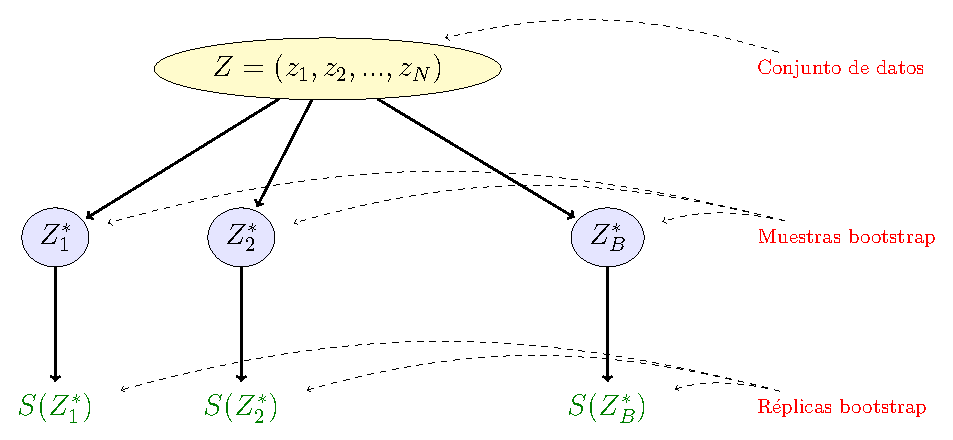
\includegraphics[width=1.1\linewidth]{gfx/chap4/untitled}}        
  \caption{Esquema del proceso bootstrap. A partir del conjunto de datos original $\mb{Z}$ se generan $B$ conjutos más, cada uno muestreando con reemplazo $N$ elementos del conjunto original. A cada uno de estos $b$ elementos se le denomina $\mb{Z}^{*}_b$, y es a partir de este que se calcula el estadístico de interés, y se le denomina réplica bootrstrap.}
  \label{fig:bootesq}
\end{figure}

%%!TEX root = ../Thesis.tex

\usetikzlibrary{arrows,shapes,positioning,shadows,trees}

\usetikzlibrary{arrows}
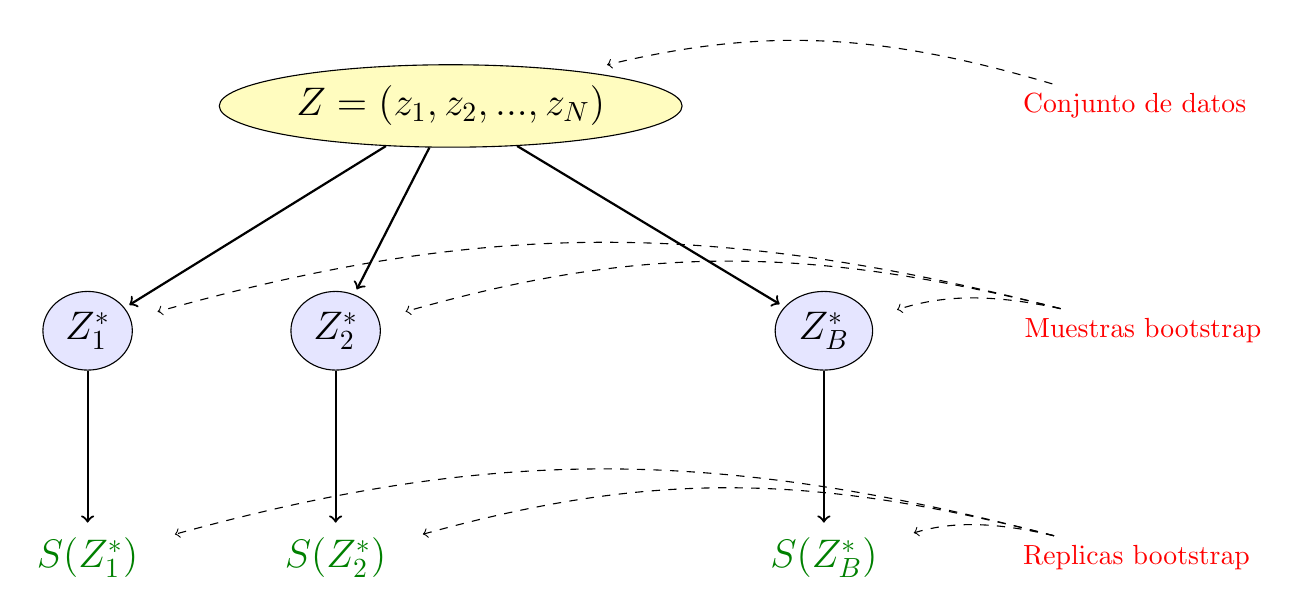
\begin{tikzpicture}[
  node distance = 1cm, auto,font=\sffamily\Large\bfseries,
  % STYLES
  every node/.style={node distance=3cm},
  % OWNs
  znode/.style={ellipse,fill=blue!10,draw},
  snode/.style={draw=none,fill=none,text=black!50!green},
  comme/.style={draw=none,fill=none,text=red,font=\normalsize}]

  \node[znode, fill=yellow!25] (main) {$Z = (z_1, z_2, ..., z_N)$};
  	\node[znode] [below left={3cm} of main](z1) {$Z^{*}_1$};
    \node[znode] [right=2cm of z1](z2) {$Z^{*}_2$};
    \node[znode] [right=5cm of z2](zb) {$Z^{*}_B$};
    
  \node[snode] [below=2cm of z1](sz1) {$S(Z^{*}_1)$};
  \node[snode] [below=2cm of z2](sz2) {$S(Z^{*}_2)$};
  \node[snode] [below=2cm of zb](szb) {$S(Z^{*}_B)$};
  
  \node[comme] [right=4.2cm of main](c1) {Conjunto de datos};
  \node[comme] [right=1.8cm of zb](c2) {Muestras bootstrap};
  \node[comme] [right=1.6cm of szb](c3) {Replicas bootstrap};
  
  \path[->,thick,shorten >=2pt]
    (main) edge (z1)
  	(main) edge (z2)
	  (main) edge (zb)
  	(z1) edge (sz1)  
    (z2) edge (sz2)  
    (zb) edge (szb);
    
  \path[dashed, ->, thin, bend right=15, shorten >= 10pt]
  	(c1) edge (main)
    (c2) edge (z1)
    (c2) edge (z2)
    (c2) edge (zb)
  	(c3) edge (sz1)
    (c3) edge (sz2)
    (c3) edge (szb);  
\end{tikzpicture}

\subsection{Bootstrap paramétrico}

\section{Selección de modelo usando bootsrap con likelihood ratio testing}

Para realizar esto, primero se usará la técnica conocida como bootstrap paramétrico para comparar el modelo correspondiente de $d$ estados contra el de $d+1$ estados ocultos.

La prueba que se realiza es comparando el \ac{MLE} $\hat \theta^{(d)}$ y $\hat \theta^{(d+1)}$ de los modelos de $d$ y $d+1$ estados respectivamente. Para la comparación se usa la estadística \ac{LLR} que corresponde a la diferencia de las log-verosimilitudes mencionadas
\begin{equation}
  LR^{(d)}_{obs} = log \frac{L(\hat \theta^{(d+1)}; y_{1:n})}{L(\hat \theta^{(d)}; y_{1:n})} =
    log L(\hat \theta^{(d+1)}; y_{1:n}) - 
    log L(\hat \theta^{(d)}; y_{1:n})
\end{equation}

Para calcular el \ac{MLE} de un modelo, se estimó la verosimilitud varias veces con diferentes parámetros iniciales aleatorios. Se iteró el algoritmo \ac{EM} hasta convergencia, un numero $iter_{hmm}$ fijo de iteraciones, esto para evitar el estancamiento del algoritmo en un máximo local, y obtener así una buena estimación de la máxima verosimilitud del modelo.

Se usó entonces como \ac{MLE} del modelo la máxima verosimilitud correspondiente a los mejores parámetros estimados y que se denotó por $LLR_{obs}$.

Ahora, para hacer la prueba con boostrap, simularemos 

\begin{algorithm}[tp]
   \caption{Muestreo ancestral para un HMM}
   \label{alg:ancsamp}
\begin{algorithmic}
   \STATE {\bfseries Input:} \\
   núm. de estados $N$, núm. de muestras en el tiempo $T$ \\
   núm. de posibles valores en el diccionario $K$, \\
   $ \pi \in \mathcal{R}^{N}; ~~ \pi_j = p(z_{1j})$ \\
   $ \mathbf{A} \in \mathcal{R}^{N \times N}; ~~
   \mathbf{A}_{jk} = p(z_{nk} \,|\, z_{n-1, j})$ \\

   $ \mathbf{E} \in \mathcal{R}^{K \times N}; ~~
   \mathbf{E}_{jk} = p(x_{nk} \,|\, z_{n, j})$\\  
   \STATE
   \STATE $z_1 \sim Multinomial(\pi)$   
   \STATE $x_1 \sim Multinomial(\mathbf{E}_{[z_1,~:]})$

   \FOR{$i = 1 \to T$} 
    \STATE $z_t \sim Multinomial(\mathbf{A}_{[z_{t-1},~:]})$ 
    \STATE $x_t \sim Multinomial(\mathbf{E}_{[z_t,~:]})$
   \ENDFOR   
\end{algorithmic}
\end{algorithm}

\section{Selección de modelo usando BIC}

Otra manera de realizar la selección del modelo que mejor se adecua a los datos que se observan, es usar una métrica específica para la selección de modelos.

%%%%%%%%%%%%

Puesto que consideramos que dentro de nuestro espacio de modelos propuestos se encuentra el modelo solución (esto es, hay un modelo que corresponde con el número de interlocutores que participan en la grabación), resulta más natural usar \ac{BIC}.

Este criterio se calcula de la siguiente manera: 
\begin{equation}
BIC(M) = 2 log-likelihood_{max}(M) - (log n ) dim(M)
\end{equation}
para cada propuesta de modelo $M$, donde $dim(M)$ es el número estimado de parámetros libres que le corresponden, y $n$ es el tamaño de nuestra muestra de datos.

Para estimar el número de parámetros libres de nuestro modelo, se consideran todas las probabilidades que rigen al \ac{HMM}, que en este caso son: la matriz a priori o inicial, la matriz de transiciones entre los interlocutores, así como la matriz de emisión de cada persona para todo el diccionario de palabras.

Esta selección se enfoca en escoger el candidato modelo con la mayor probabilidad dados los datos, pero penalizando la complejidad de cada propuesta. Se preferirán entonces los modelos con una mayor verosimilitud que involucren la menor cantidad de parámetros posibles. 

...